%this file is the second report
%a % comment anything after % until the end of the line

%minimum references to begin our article
\documentclass[12pt]{article}
\usepackage[english]{babel}
\usepackage[utf8]{inputenc}
\usepackage[T1]{fontenc}
\usepackage{graphicx}
\usepackage{fancyhdr}
\usepackage{hyperref}
\usepackage{float}
\usepackage{enumitem}
\usepackage{amsmath}
\usepackage[margin=1in]{geometry}
\usepackage{indentfirst}
\usepackage{titlesec}
\usepackage{verbatim}
\usepackage{url}
\newcommand{\sectionbreak}{\clearpage}

%\setlength{\parskip}{10pt plus 1pt minus 1pt} %Adds spacing between paragraphs 
\usepackage{parskip}
\setlength{\parindent}{15pt}

\pagestyle{fancy}
%\cfoot{Fast and furious game playing: Monte Carlo drift}
% the last extension makes it possible to add images

%presentation of the document
\title{Fast and Furious Game Playing: Monte Carlo Drift\smallbreak Specifications report} %not sure about the name of this report
\author{Prateek \textsc{Bhatnagar}, Baptiste \textsc{Bignon}, \\
        Mikaïl \textsc{Demirdelen}, Gabriel \textsc{Prevosto}, \\
        Dan \textsc{Seeruttun-{}-Marie}, Benoît \textsc{Viguier} \\
        \\
        Supervisors: Nikolaos \textsc{Parlavantzas}, Christian \textsc{Raymond}}
\date{11/27/2014}
\setlength\parindent{15pt}
\begin{document}
\maketitle

\begin{figure}[!h] 
\centerline{\includegraphics[scale=0.50]{Pictures/arimaa}}
\end{figure}
\newpage


\begin{abstract}
%put abstract here
	Insert text here
\end{abstract}
\newpage

%to add a table of contents
\tableofcontents
\newpage


\section{Introduction}						\label{sec:introduction} 		
Our project is called Fast and furious game playing, MonteCarlo drift. Our purpose is to create an Artificial Intelligence able to compete against humans using the MonteCarlo Tree Research.
\newline
We will only focus on two players games. Furthermore, we want to avoid games already resolved. We will choose something not studied entirely. We want to work on some new application. That is why we are interested by Arimaa.
\newline
\newline
For our game, we will need a program and statistics to make a good Artificial Intelligence. Each move should be calculated using a reliable method.
MonteCarlo Tree Research is an algorithm able to take these optimal decisions. It has been used in the past for draughts, or chess. By exploring numerous possibilities, it will become possible to know what move is the better one.
We will parallelize this algorithm in order to use it in a multi-core machine, to improve his efficiency.
That MCTS algorithm is better than the classic Min-Max algorithm, that is why we will use it.
\newline
\newline
We will analyse parallelization methods, we will present it, and then we will choose the one adapted to our project.
Thanks to the results of these latest methods, we will be able to choose a state resulting of the current move. Then we will explore the tree and with the same methods as before, we will figure out what the opponent will most probably do. The way we will be exploring the tree will only depend on the parallelization method.
The first part of our project will be the analysis of latest thesis of technologies we will use, in order to choose the best one, and using it on the right environment, to improve his  efficiency.
In the next part, we will choose technologies we will need to achieve our goals, we will create a UML diagram to settle down our program.
\newline
\newline
Finally, in the last part, we will implement this program, and its documentation and test his executing on Grid5000, a cluster of multi-core machines.
What is interesting in this project is we will create an Artificial Intelligence using technologies and methods fully optimized. Then we will create a program that can lead to true improvements for current algorithms applied to this game.



\newpage

\section{Algorithmic methods}
An explanation of our methods and concepts is necessary to understand how our project works. The use of some parallelization methods, and the MCTS algorithm is here developed.					\label{sec:algorithmicMethods}
	\subsection{Parallelization methods}			\label{sec:parallelization}		In order to increase the speed of our program, we have decided to parallelize it on a set of cluster of multicore machines. But there is many ways of parallelize our algorithm and we have to choose how we want to do it. 
\subsection{Previous Work}
In the last report, we talked about the different methods, their advantages and drawbacks. We have seen that there is mainly two parallelization methods that are efficient.
\newline
The first one is called the Root Parallelization. It consists in giving the tree to develop to every threads, let them develop it randomly without any communication with the environment
during a certain amount of time and then, merge the results of each tree.
This method has the great benefit of reducing at maximum the communication between the actors, in this case, the threads.
There's only a communication at the beginning and at the end, without needing any synchronization. The Root Parallelization is depicted in figure \ref{root}.
\newline
The other efficient parallelization method is called UCT-Treesplit. It looks like Root Parallelization as we give to each actor the same tree to develop.
Contrary to Root Parallelization, when the tree is develop on certain node, it goes on working packages who are distributed among every actor.
In terms of performance, this method is very efficient but need an High-Performance Computer, or HPC, and is very sensitive to network latency.
\newline
We have to choose two parallelization methods, one for the cluster parallelization and another for the shared memory parallelization.
\subsection{Cluster Parallelization}
For the cluster parallelization, we have to take into account the fact that we will need to communicate by sending messages, so it is relatively costly.
Moreover, as the network can have latency we should minimize the communication between the computers and that's why we have choose to implement a Root Parallelization.
It reduces the cost in communication at maximum, is very simple to implement,it does not depend of configuration of each computer and is very efficient.
\subsection{Shared Memory Parallelization}
For the shared memory parallelization we could choose both Root Parallelization or UCT-Treesplit.
If we choose UCT-Treesplit, we may not success to implement it correctly since it is a very complex strategy and, moreover, it may not be perfect BLA BLA BLA.

	\subsection{\textit{Monte Carlo Tree Search algorithm}}		\label{sec:mcts}			\subsection{The Minimax algorithm}
% miss the blank space
The Minimax algorithm is a way of finding an optimal move in a two player game. In the search tree for a two player game, there are two kinds of nodes, nodes representing ones moves and nodes representing the opponent's moves.\cite{graphics_minimax}
\begin{figure}[H]
\centering
	\begin{minipage}[b]{0.45\linewidth}
		\centering
		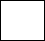
\includegraphics[height=1cm]{2_State_of_the_art/Arimaa_on_MCTS_Benoit/img/max.png}
		\caption{\label{fig:max}Nodes representing ones moves are generally drawn as squares, these are also called \emph{MAX} nodes.}
	\end{minipage}%
	\hspace*{1cm}
	\begin{minipage}[b]{0.45\linewidth}
		\centering
		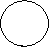
\includegraphics[height=1cm]{2_State_of_the_art/Arimaa_on_MCTS_Benoit/img/min.png}
		\caption{\label{fig:min}Nodes representing the opponent's moves are generally drawn as circles, these are also called \emph{MIN} nodes.}
	\end{minipage}%
\end{figure}

The goal of a \emph{MAX/MIN} node is to maximize/minimize the value of the subtree rooted at that node. To do this, a \emph{MAX/MIN} node chooses the child with the greatest/smallest value, and that becomes the value of the \emph{MAX/MIN} node.

Note that it's typical for two player games to have different branching factors at each node. The move one makes could have an impact on what moves are possible for the opponent. In this example, one is ignoring what the game is in order to focus on the algorithm.

\begin{figure}[H]
\centering
	\begin{minipage}[b]{0.45\linewidth}
		\centering
		\includegraphics[height=1.5cm]{2_State_of_the_art/Arimaa_on_MCTS_Benoit/img/Minimax2.png}
		\caption{\label{fig:Minimax2}At the start of the problem, Minimax checks the single present node.}
	\end{minipage}%
	\hspace*{1cm}
	\begin{minipage}[b]{0.45\linewidth}
		\centering
		\includegraphics[height=3cm]{2_State_of_the_art/Arimaa_on_MCTS_Benoit/img/Minimax3.png}
		\caption{\label{fig:Minimax3}It begins like a depth first search, generating the first child.}
	\end{minipage}%
\end{figure}

So far we've really seen no evaluation values. The way Minimax works is to go down a specified number of full moves (where one \emph{full move}' is actually a move by each player), then calculate the evaluation values for states at that depth. For this example, we're going to go down one full move, which is one more level.
\begin{figure}[H]
\centering
	\begin{minipage}[b]{0.45\linewidth}
		\centering
		\includegraphics[height=3cm]{2_State_of_the_art/Arimaa_on_MCTS_Benoit/img/Minimax4.png}
		\caption{\label{fig:Minimax4}we generate the values for those nodes.}
	\end{minipage}%
	\hspace*{1cm}
	\begin{minipage}[b]{0.45\linewidth}
		\centering
		\includegraphics[height=3cm]{2_State_of_the_art/Arimaa_on_MCTS_Benoit/img/Minimax5.png}
		\caption{\label{fig:Minimax5}It chooses the minimum of the two child node values, which is 3.}
	\end{minipage}%
\end{figure}

The max node at the top still has two other children nodes that we need to generate and search.

\begin{figure}[H]
\centering
	\begin{minipage}[b]{0.45\linewidth}
		\centering
		\includegraphics[height=3cm]{2_State_of_the_art/Arimaa_on_MCTS_Benoit/img/Minimax6.png}
		\caption{\label{fig:Minimax6}Since there is only one child, the min node must take it's value.}
		\end{minipage}%
	\hspace*{1cm}
	\begin{minipage}[b]{0.45\linewidth}
		\centering
		\includegraphics[height=3cm]{2_State_of_the_art/Arimaa_on_MCTS_Benoit/img/Minimax8.png}
		\caption{\label{fig:Minimax8}The third min node chooses the minimum of it's child node values, 1.}
	\end{minipage}%
\end{figure}

Finally we have all of the values of the children of the max node at the top level, so it chooses the maximum of them, 15, and we get the final solution. 

\begin{figure}[H]
\centering
	\begin{minipage}[b]{1\linewidth}
		\centering
		\includegraphics[height=3cm]{2_State_of_the_art/Arimaa_on_MCTS_Benoit/img/Minimax9.png}
		\caption{\label{fig:Minimax9}Final tree.}
	\end{minipage}%
\end{figure}

What this tells us is that we should take the move that leads to the middle min node, since it'll lead to the best possible state for us one full move down the road.

\subsection{The \ensuremath{\alpha\beta} pruning} %pruning = elaguage en anglais
The \ensuremath{\alpha\beta} method is a heuristic that decrease the number of leaf that will be explored by the Minimax algorithm. That way, the size of the tree will be smaller, the algorithm will be able to dive further and the time spend on more interesting subtree is greater.\\
If the leaf's position is less interesting than its parents, the algorithm won't explore anyfurther.

\subsection{Monte Carlo Tree Search Algorithm}
\subsubsection{Introduction}
Monte Carlo Tree Search (MCTS) is an algorithm used for taking decisions in Artificial Intelligence (AI) problems such as solving games or decision making in project managment. It is based on making a big number of random simulations in order to get trustfull datas. To make such simulations, the program play the moves randomly for each players. Once it reach a conclusion (win or loss), the program compute the statistics to get the odds of winning.
\subsubsection{How does it works ?}
The Algorithm create a tree with all possible solution with a small depth.
Then it start to run random simulations starting from the leaves in order to test the odds of the outcome.
Once we got enough the results (usually we are using time based simulations) we feed back the results and make the decision depending on the odds of each subsequent leaves.
\subsubsection{Example}
\label{sec:example}
\begin{figure}[H]
\centering
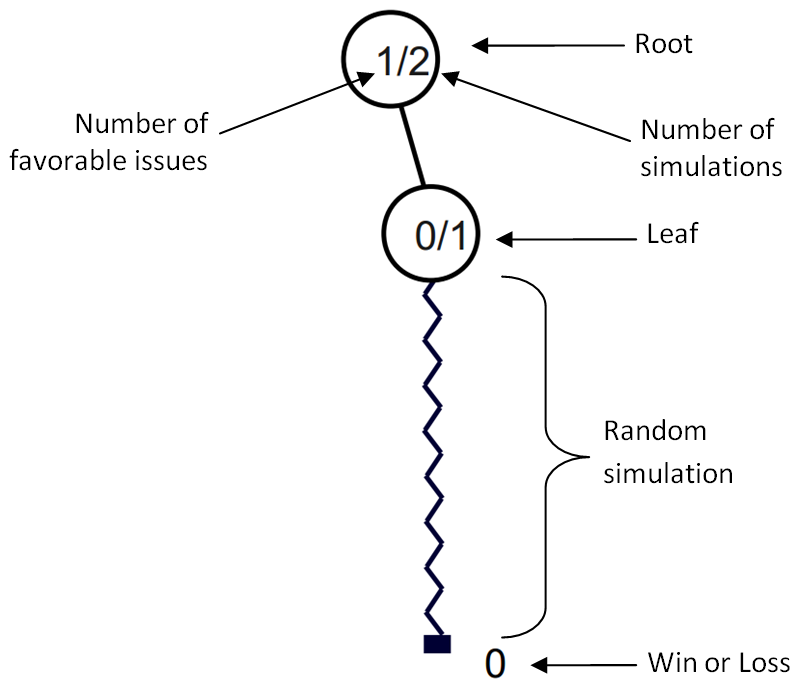
\includegraphics[height=5cm]{1_Presentation/1.2_Algorithm_MCTS_Benoit/img/schema.png}
\caption{\label{fig:schema}Legend of the following figures.}
\end{figure}

\begin{figure}[H]
\centering
	\begin{minipage}[b]{0.45\linewidth}
		\centering
		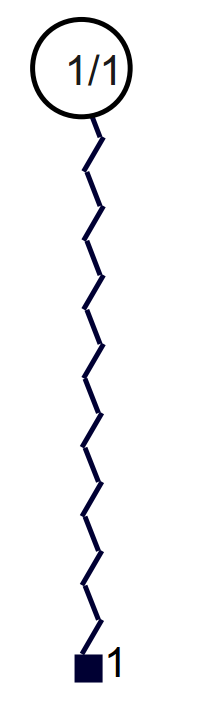
\includegraphics[height=4cm]{1_Presentation/1.2_Algorithm_MCTS_Benoit/img/1.png}
		\caption{\label{fig:1}Run a first simulation from the root, get a favorable issue (will be considered as a \textit{win}).}
	\end{minipage}%
	\hspace*{1cm}
	\begin{minipage}[b]{0.45\linewidth}
		\centering
		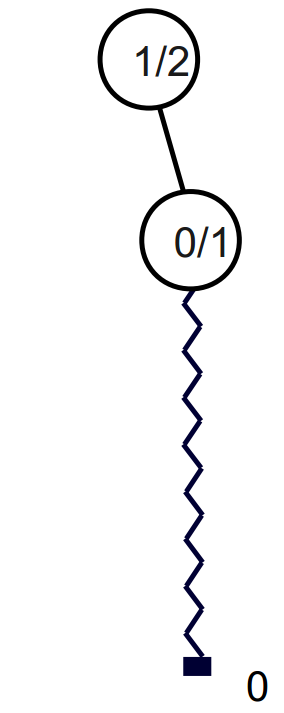
\includegraphics[height=4cm]{1_Presentation/1.2_Algorithm_MCTS_Benoit/img/2.png}
		\caption{\label{fig:2}Create a first leaf at depth 1 and run the simulation, get an unfavorable issue (considered as a \textit{loss}).}
	\end{minipage}%
\end{figure}

\begin{figure}[H]
\centering
	\begin{minipage}[b]{0.3\linewidth}
		\centering
		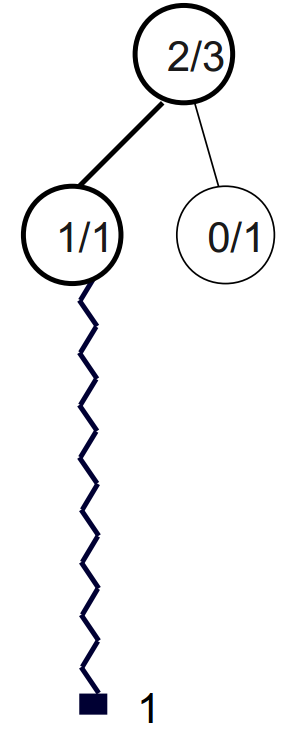
\includegraphics[height=4cm]{1_Presentation/1.2_Algorithm_MCTS_Benoit/img/3.png}
		\caption{\label{fig:3}Create a second leaf at depth 1 and run the simulation (\textit{win}).}
	\end{minipage}%
	\hspace*{1cm}
	\begin{minipage}[b]{0.3\linewidth}
		\centering
		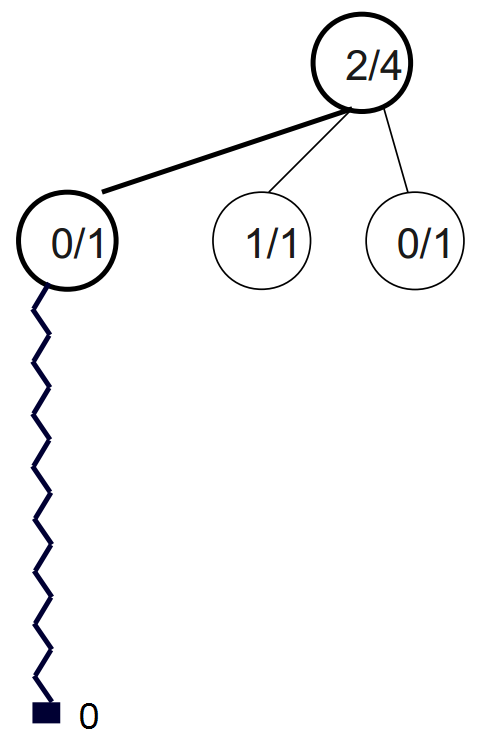
\includegraphics[height=4cm]{1_Presentation/1.2_Algorithm_MCTS_Benoit/img/4.png}
		\caption{\label{fig:4}Create a third leaf at depth 1 and run the simulation (\textit{loss}).}
	\end{minipage}%
	\hspace*{1cm}
	\begin{minipage}[b]{0.3\linewidth}
		\centering
		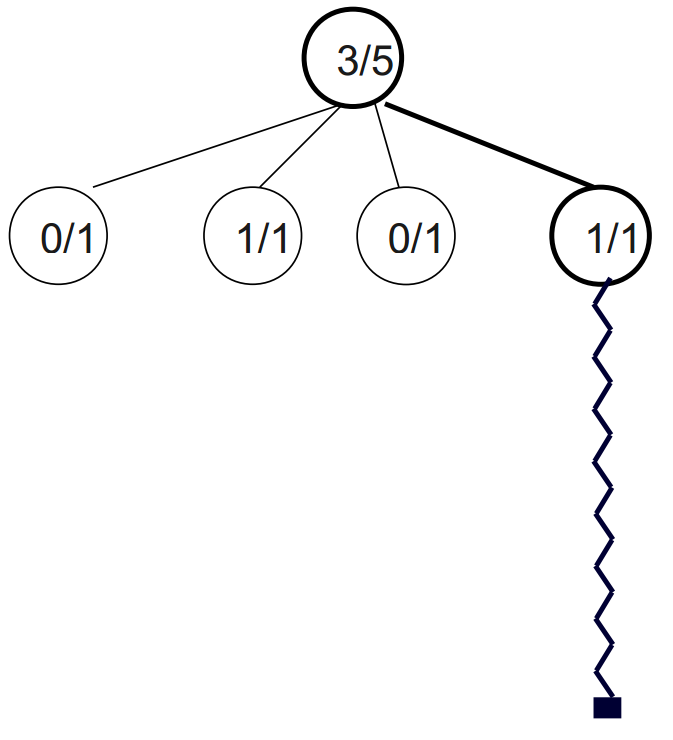
\includegraphics[height=4cm]{1_Presentation/1.2_Algorithm_MCTS_Benoit/img/5.png}
		\caption{\label{fig:5}Create a fourth leaf at depth 1 and run the simulation (\textit{win}).}
	\end{minipage}%
\end{figure}

Right now the odds of winning are 3/5. Now that we tested all the possible outcomes at depth 1, we will expend the tree on the favorable leaves (here the second and fourth).

\begin{figure}[H]
\centering
	\begin{minipage}[b]{0.45\linewidth}
		\centering
		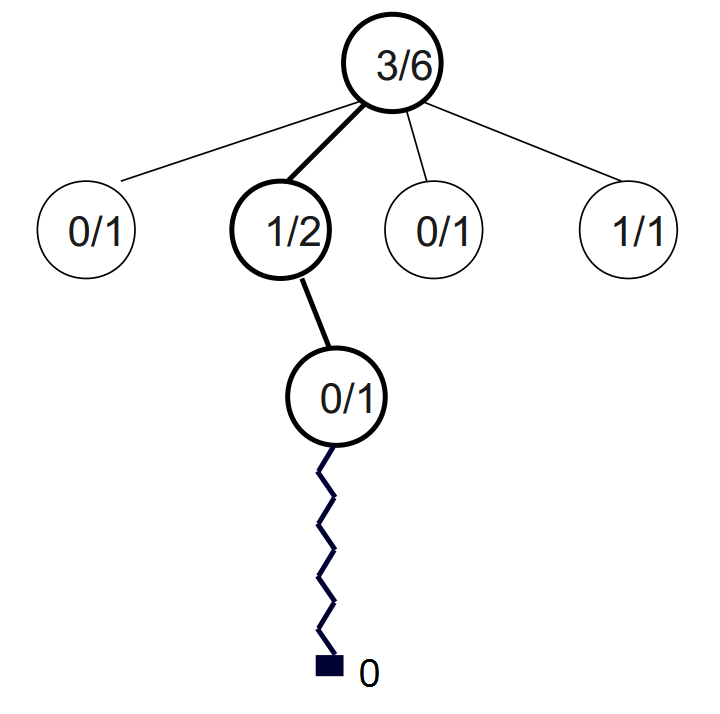
\includegraphics[height=4cm]{1_Presentation/1.2_Algorithm_MCTS_Benoit/img/6.png}
		\caption{\label{fig:6}Create a leaf at depth 2 with parent the 2nd leaf at depth 1 and run the simulation (\textit{loss}), update the odds value of the node and making it less interesting than the fourth node. Therefore the algorithm will now work on the fourth node.}
	\end{minipage}%
	\hspace*{1cm}
	\begin{minipage}[b]{0.45\linewidth}
		\centering
		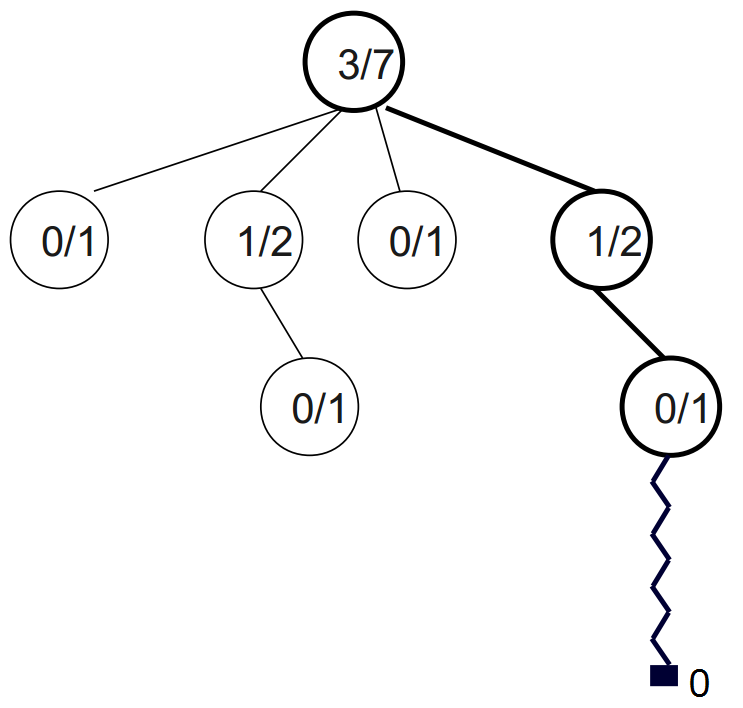
\includegraphics[height=4cm]{1_Presentation/1.2_Algorithm_MCTS_Benoit/img/7.png}
		\caption{\label{fig:7}Create a leaf at depth 2 with parent the fourth leaf at depth 1 and run the simulation (\textit{loss}), update the odds value of the node and making it as interesting as the second node. The algorithm will now work on the second node.}
	\end{minipage}%
\end{figure}
\begin{figure}[H]
\centering
	\begin{minipage}[b]{0.45\linewidth}
		\centering
		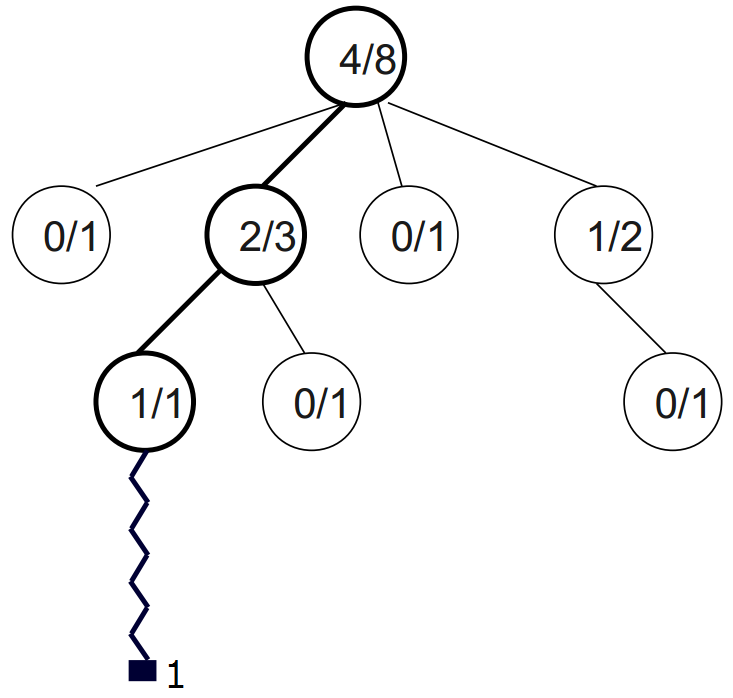
\includegraphics[height=4cm]{1_Presentation/1.2_Algorithm_MCTS_Benoit/img/8.png}
		\caption{\label{fig:8}Create a second leaf at depth 2 with parent the second leaf at depth 1 and run simulation (\textit{win}), update the odds value and continue to develop this leaf.}
	\end{minipage}%
	\hspace*{1cm}
	\begin{minipage}[b]{0.45\linewidth}
		\centering
		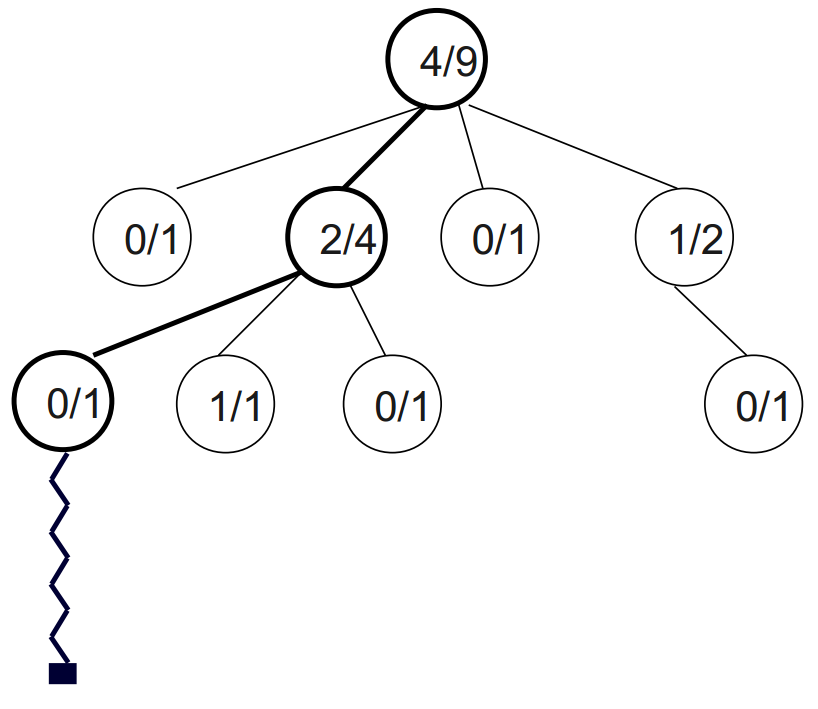
\includegraphics[height=4cm]{1_Presentation/1.2_Algorithm_MCTS_Benoit/img/9.png}
		\caption{\label{fig:9}Create a third leaf at depth 2 with parent the second leaf at depth 1 and run simulation (\textit{loss}), update the odds value and switch to the fourth leaf.\null\\}
	\end{minipage}%
\end{figure}

Continue the Algorithm until a decent about of simulation are run and/or the time limit is .
\begin{figure}[H]
\centering
	\begin{minipage}[b]{0.33\linewidth}
	\centering
		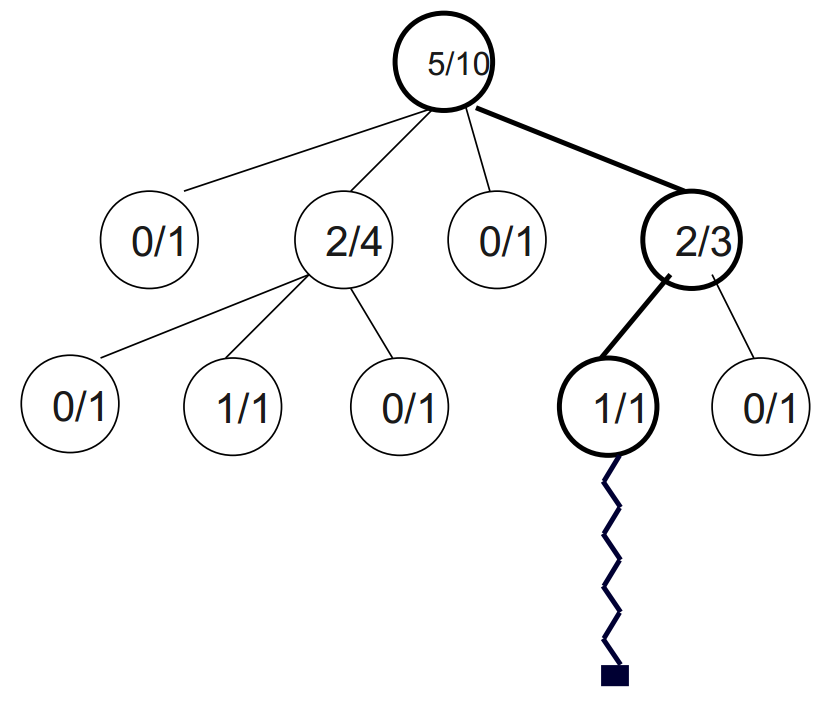
\includegraphics[height=4cm]{1_Presentation/1.2_Algorithm_MCTS_Benoit/img/10.png}
	\end{minipage}%
	\begin{minipage}[b]{0.33\linewidth}
	\centering
		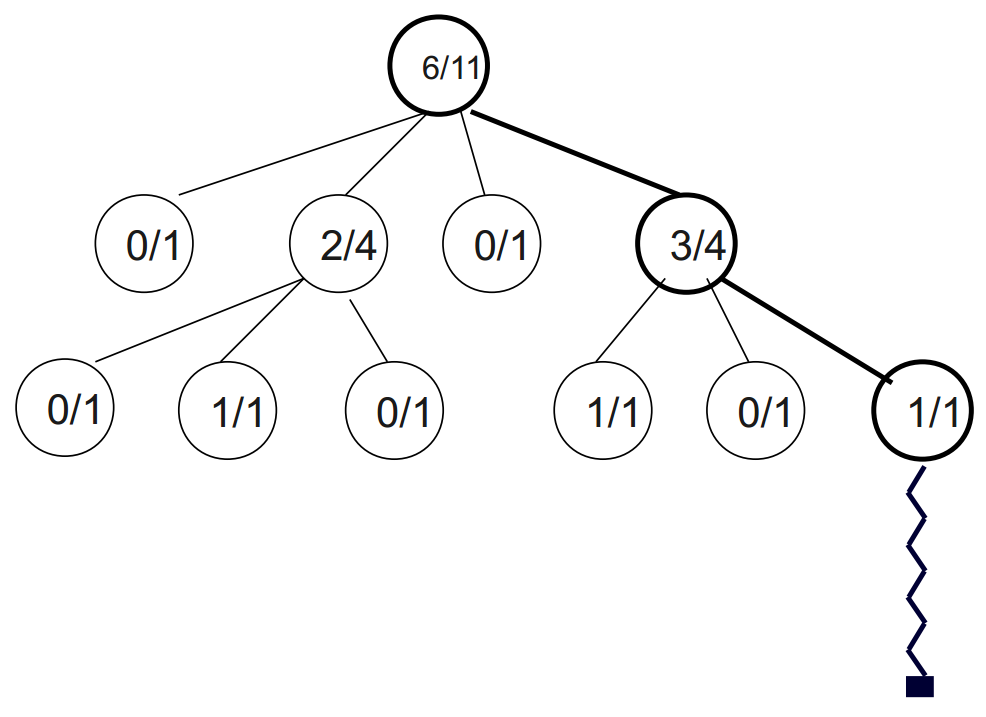
\includegraphics[height=4cm]{1_Presentation/1.2_Algorithm_MCTS_Benoit/img/11.png}
	\end{minipage}%
	\begin{minipage}[b]{0.33\linewidth}
	\centering
		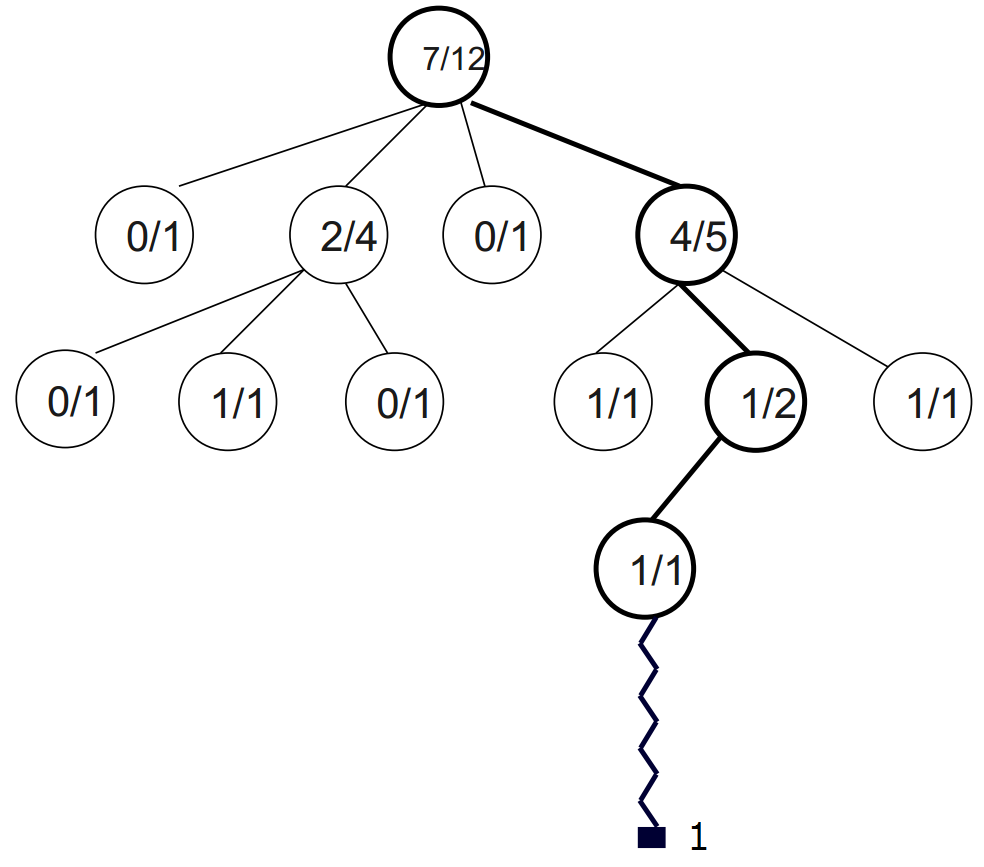
\includegraphics[height=4cm]{1_Presentation/1.2_Algorithm_MCTS_Benoit/img/12.png}
	\end{minipage}%
\end{figure}

Make a decision : here we chose the fourth leaf.\\
\newpage
\subsubsection{How to select the leaves to develop ?}
In the previous exemple, we chose to not expend leaves without winrates. But depending on the results of the simulations, wins can vary greatly. Therefore we will run more simulations on each leaf before chosing the ones to develop. For practical purpose we will select the leaves to expend that has the highest value of the cost function UCT (Upper Confidence Bound 1 applied to Trees).\\
\bigskip
\begin{minipage}[b]{1\linewidth}
\centering
\begin{equation*}
f = \frac{w_i}{n_i} + c\sqrt{\frac{\ln t}{n_i}}
\end{equation*}
\medskip
\textit{UCT function}\cite{formula_UCT}

\end{minipage}%
\bigskip
\begin{itemize}
  \item \ensuremath{w_i} : number of wins after the ith node
  \item \ensuremath{n_i} : number of simulations after the ith node
  \item \ensuremath{c}   : exploration parameter – theoretically equal to \ensuremath{\sqrt{2}} but in practice chosen empirically
  \item \ensuremath{t}   : total number of simulations in a given tree node, equal to the sum of all \ensuremath{n_i}
\end{itemize}
\medskip
The more a leaf is developed, the less it's cost is worth it. This way we can be sure that a leaf with low winrate isn't completely forgotten.\\

\subsubsection{Why using the Monte Carlo Tree Search ?}
 The advantage of MCTS with it's basic form is that you don't need to implement functions to improve the researches. Based on its random simulations, it will determine by itself which are the good options and which aren't.\\ The more you run simulations, the more accurate the results will be.

\subsubsection{How much power do we need ?}
The more the game has possible moves, the more power it require to solve. In order to get decisions, it needs to go deeper in the tree and to search enough leaves. If the time or number of simulations is not sufficient, the algorithm might miss some important branches and fail to give plausible results. Therefore in order to get decent results, using high-end computer is mandatory, it allows us to get access to multi-threading technology in order to parallelize the simulations.
\newpage

\section{General Architecture}					\label{sec:generalArchitecture} 		
	\subsection{Introduction}			\label{sec:gameBehavioiur}		In order to test the AI\footnote{Artificial Intelligence}, an application will be developped.
This application will include a two-player mode, a one-player mode and a demonstration mode (AI versus AI).
In the case where several AI have been implemented, the user will be able to choose which one to play against.

\begin{figure}[!h]
\centering
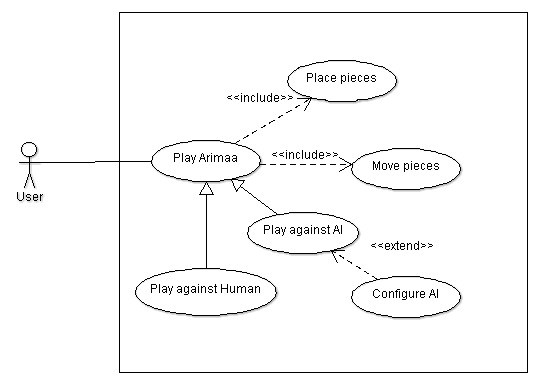
\includegraphics[width=\textwidth]{2General_Architecture/2.1Behaviour_of_the_Game/Pictures/Application_UCD}
\caption{The user-case diagram describing the application}
\label{fig:UCD_Play}
\end{figure}

In order to make the game easy to play, this application will provide a graphical User Interface (further referred to as \emph{UI}). % as described in part ??
This UI, as well as the algorithm for the AI, will act upon the game model, so as to inform it of what moves were made.
The UI will also regularly update to give the player feedback on the progression of the game.

	\subsection{Context of the architecture}		\label{sec:globalview}			The organization of the architecture is described in Figure \ref{fig:gra}.

First a module User Interface will be used by the user to play the game. Then the User Interface will transmit the data to the module Model. The model is able to make the move, to update the board. If the game is a human game, the Model will only interact with the User Interface. Otherwise, for the computer move, it will communicate with the MCTS module via the API. This API is here to make communicate the Model and the MCTS module. The MCTS is using an implementation of the parallelization to compute his algorithm faster, using different computers.

\begin{figure}[!h]
\centering
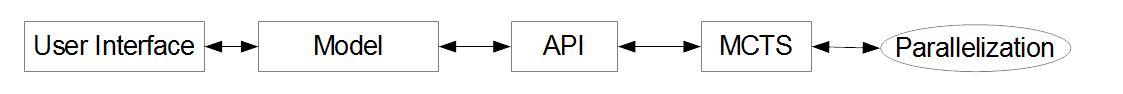
\includegraphics[width=1\textwidth]{2General_Architecture/2.1.2GeneralView/graphe2.png}
\caption{General view of the architecture}
\label{fig:gra}
\end{figure}


Here is a diagram showing the links between the interface and the rest of the modules in Figure \ref{fig:gen}

\begin{figure}[!h]
\centering
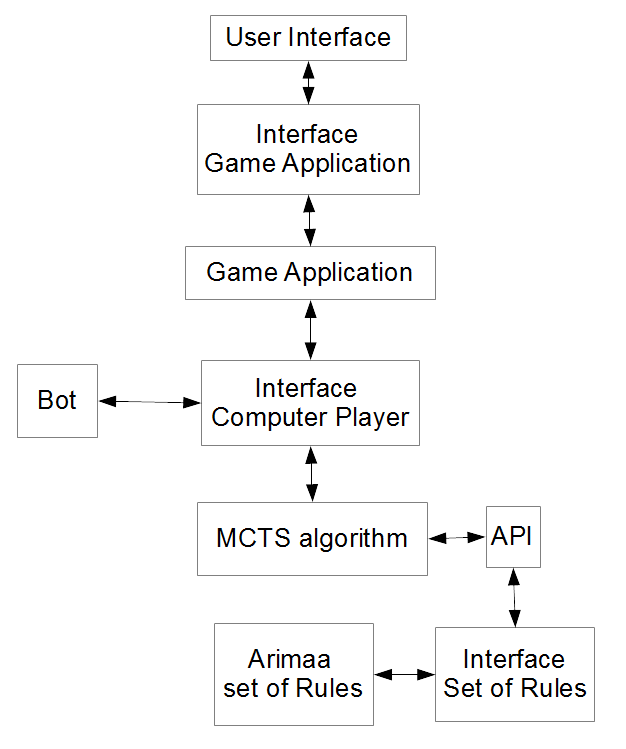
\includegraphics[width=0.5\textwidth]{2General_Architecture/2.1.2GeneralView/gen.png}
\caption{Interfaces of the architecture}
\label{fig:gen}
\end{figure}

The user will interact with the user interface, which will communicate with the game application, where all data for the game will be stored. Then, it will communicate with an Interface which will handle the communications between the Game application and the computer player. 

In our case, the computer player will be played by the AI using the MCTS algorithm, communicating with the Arimaa set of rules via the API and an interface for the set of Rules.  If another algorithm is to be tested, it will be added.

Interfaces are very important because they make it possible for others to use our project for others games than Arimaa without rebuilding everything. They would only have to implement the Interface with their proper game, game rules.

Furthermore, if the time permits it, the management of computers bots\footnote{For instance of the site \textit{Arimaa.com}} will be added. The only problem here is the computers bots are not similar to each other, thus it will take time to implement a class which will be able to communicate with both the computer bot and the interface.

The input of our software will be provided by the user using the mouse and keyboard. The output will only be the display of the screen, after the computer player makes a move.
	\subsection{User Interface module}				\label{sec:ui}				In order to test our program against human players, we will develop an application implementing a graphical user interface (\emph{GUI} or also \emph{UI}).
Figure \ref{fig:UCD_Play} represents the interactions between the player and the UI.
It will interface directly with the model, and will be controllable by the human with the mouse or keyboard, in a manner as intuitive as possible.
Thanks to this UI, the user will be able to choose between a one-player mode, a two-plaer mode and a demonstration mode.
This last mode consists in a match between two AIs, and will be helpful to compare different AIs.
The user will also be able to choose and configure the AIs, if we have time to develop more than one.

\begin{figure}[H]
\centering
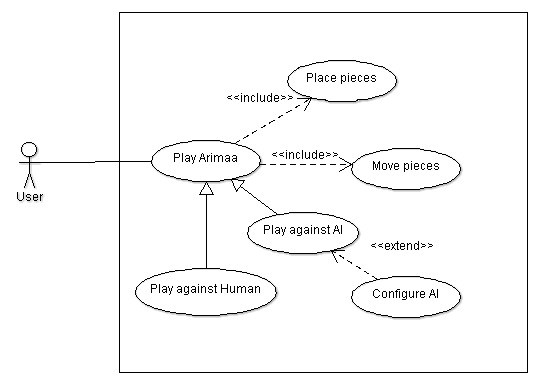
\includegraphics[width=\textwidth]{2General_Architecture/2.1Behaviour_of_the_Game/Pictures/Application_UCD}
\caption{The user-case diagram describing the interactions made possible by the UI}
\label{fig:UCD_Play}
\end{figure}
	\subsection{Converter module}		\label{sec:api}				API stands for Application Programming Interface. An API is a set of routines, protocols, and tools for building software applications. The API specifies how software components should interact and are used when programming graphical User Interface (GUI) components. A good API makes it easier to develop a program by providing all the building blocks. A programmer then puts the blocks together.

 In this project the API will be induced between the MCTS algorithm and the board game application. It will be responsible for providing the input to the board game application in understandable format and will receive the input from the MCTS algorithm. Its usage is described in figure \ref{fig:flowchart}.

\bigbreak

\begin{figure}[H]
	\centering
	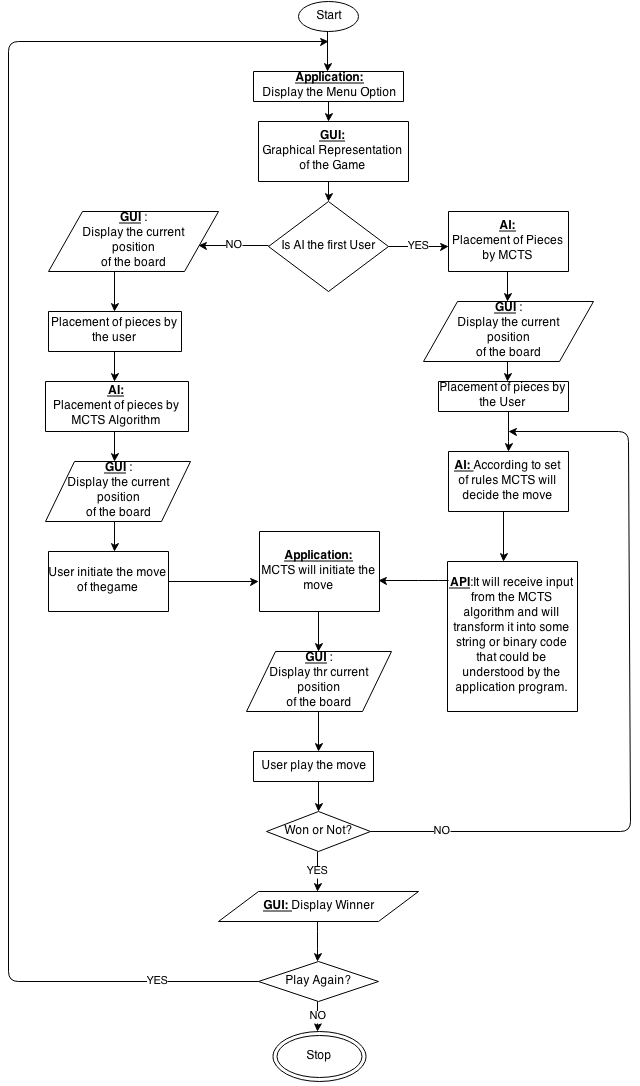
\includegraphics[width=\textwidth]{2General_Architecture/2.2API/img/DiagramAPI.png}
	\caption{The flowchart describing the usage of the API}
	\label{fig:flowchart}
\end{figure}



	\subsection{The MCTS algorithm module}		\label{sec:mctss}				The next Figure \ref{fig:flow} describes the AI, i.e. the MCTS Algorithm module.

\begin{figure}[H]
	\centering
	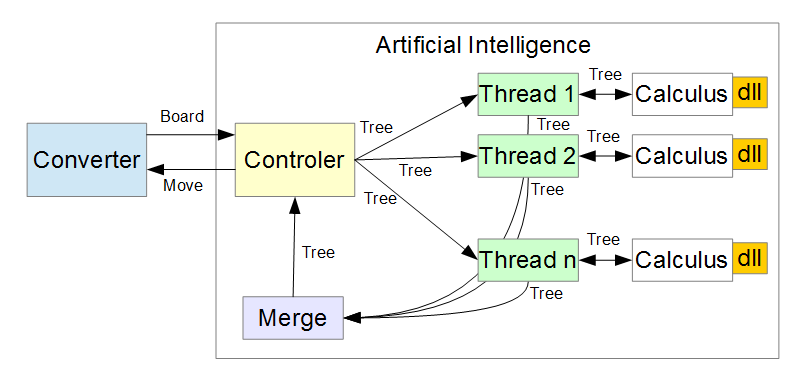
\includegraphics[width=0.80\textwidth]{2General_Architecture/2.3MCTS/AI.png}
	\caption{Block Diagram of Converter}
	\label{fig:flow}
\end{figure}

The converter sends the state of the board to the controler, which creates trees in different threads. Each of these threads computes his tree, getting the possible moves thanks to a set of rules, gathered together in a dynamic link library dll. 

Then, when the calculus is over, the thread hands over the tree to the Merge module. When all threads have done it, the module merges the trees, gathering data in an only tree, that is sent to the controler.

Finally, the controler is able to decide what move to choose and it sent this move to the converter.


\newpage

\section{Software solutions}					\label{sec:softwareSolutions}
	\subsection{Shared memory Parallelism on CPU}	\label{sec:openmp}			To parallelize our algorithm on the CPU, we need to chose a framework. Four solutions have been found and compared :
\begin{itemize}
\item MPI
\item OpenMp
\item C++11 Threads (Boost)
\item Pthreads (C)
\end{itemize}

\subsubsection{MPI}
MPI is a library mainly dedicated to parallelization between different machines, it could work on a single CPU but doesn't provide as many possibilites as its counterparts. Therefore we do not choose to do it for that part of the implementation.

\subsubsection{Pthreads}
Pthreads are out of order because they are depreciated : it is a C language library and the C++11 language provides more efficiency and possibilities. The threads management is heavy to code and requires a good knowledge of how threads works precisely.

\subsubsection{OpenMP and C++11}
OpenMP and C++11 are the only remaining options. C++11 language is a simplification of the Boost library inducing the latest to be more complete. The following table sumarizes each libraries pros and cons :
\begin{center}
\begin{tabular}{| l | l | l |}
\hline
\multicolumn{1}{| c}{OpenMP} &\multicolumn{1}{| c}{C++11 Threads} &\multicolumn{1}{| c |}{ Pthreads (C) } \\
\hline
+ Options & + Flexibility & + Flexibility \\
+ Portable & + Type-Safety & + Low-level \\
+ Languages & + Possibilities & + Compatibility \\
- Performances & - Fortran & - Efforts \\
- Memory & - Compiler & - Type-safety \\
- Unreliable & - Scalling & - Management  \\
\hline
\end{tabular}
\end{center}

Both libraries get similar performances\footnote{http://www.cs.colostate.edu/~cs675/OpenMPvsThreads.pdf}. However OpenMP is easier to use (precompilier declarations...) and keeps the code clean. C++11 language allows a better thread management. Nevertheless it can easily also fall behind his counterpart in term of speed if some mistakes are made : a high price has to be paid.

Considering OpenMP safer to use and get similar results to C++11 language, we chosed OpenMP to parallelize our algorithm on CPU\footnote{Central Processing Unit}.
	\subsection{Shared memory Parallelism on GPU}	\label{sec:openacc}			\input{4Software_Solution/4.2OpenACC/OpenACC.tex}
	\subsection{Cluster Parallelism}			\label{sec:mpi}				Our last software needed is about cluster parallelization. As we have decided to use \textit{Root Parallelization}, there will not be a lot of communication between the different computers. We can choose between two solutions: the Sockets and MPI.
\begin{itemize}
\item A socket is  a low-level mechanism used to communicate across a computer network. The socket is an end point of the communication flow.
\item MPI is a standardized message-passing system. It allows us to communicate between computers which belong to a network by sending messages between them. 
\end{itemize}
\subsubsection{The chosen solution}

We decided to use MPI for the following reasons:
\begin{itemize}
\item MPI is more high-level than the sockets, thus it will be simpler to implement in our software.
\item The community behind MPI is large so there would not be any problem to fix the different bugs. Moreover, the MPI documentation is clearer than the sockets'. 
\item MPI uses sockets so it is similar, though a little bit inferior to the sockets, in term of performance.
\end{itemize}
In conclusion, MPI would be simpler to implement, is more documented than the sockets while they both have almost similar performance. So, it seems more adapted to our project than the sockets.
	\subsection{Actor Model}				\label{sec:actorModel}			In the parts just before, three solutions are presented which permit using together to parallelize our algorithm. In this part will be quickly introduced another way to do this, the actor model.

In this model, each machine, each core and each GPU is seen as an actor. The actors can send messages amongst themselves. When they receive one, they can:
\begin{itemize}
\item send messages to other actors
\item create new actors
\item modifie their behavior
\end{itemize}

This actions can be realize in parallel. Moreover the system of message is totally asynchronus which is adapted to the root parallelization we will use at the beginning. But it will not be too interested for other parallelization methods. For the moment we have not found yet a framework implementing the actor model that we could use for our project but we are still investigating because it could be a very efficient solution. 
\newpage

\section{Conclusion}						\label{sec:conclusion}			
The main focus area of this report is planning. Various planning methods have been decided such as Agile development methodology and Planning Poker method.
Using Agile Development Methodology, the incremental  development of the project will take place. Planning Poker method  which is the estimation technique of Agile Methodology is used to estimate the time requirement for the development of the project. The dates have been estimated with respect to the development of various models of our project.A serious attempt is made analyse the risks  in order to take preventive measures to avoid various risks and problems. 

\newpage

%uncomment to add bibliography
\bibliography{bibliography}
\bibliographystyle{plain}

\end{document}
